
\documentclass[t, 11pt]{beamer}
\pdfmapfile{+sansmathaccent.map}
%%% Работа с русским языком
\usepackage{cmap}				
\usepackage{mathtext} 				
\usepackage[T2A]{fontenc}		
\usepackage[utf8]{inputenc}			
\usepackage[russian, english]{babel}	

\usetheme{Montpellier}
\usecolortheme{beaver} % Цветовая схема



%%% Работа с картинками
\usepackage{graphicx}

\usepackage{csquotes}

\hypersetup{				
	colorlinks=true,       	
	linkcolor=blue,          
	citecolor=black,       
	filecolor=magenta,      
	urlcolor=red           
}
%% табличка
\usepackage{booktabs, caption, makecell}
\usepackage{threeparttable}

%% график нормального распределения 
\usepackage{tikz}
\usepackage{xcolor}
\usepackage{pgfplots}
\pgfplotsset{compat=1.7}

%% доп символы
\usepackage{newunicodechar}

\newcommand\Warning{%
	\makebox[1.4em][c]{%
		\makebox[0pt][c]{\raisebox{.1em}{\small!}}%
		\makebox[0pt][c]{\color{red}\Large$\bigtriangleup$}}}%

\newunicodechar{⚠}{\Warning}

\title {Data Vizualization}
\subtitle{with ggplot2}
\author{Chuvakin Sergey}
\date{\today}
\institute[<<Anthropology>>]{<<School of Advanced Studies>>}

\begin{document}

	
	\frame[plain]{\titlepage}		
	
	\section{Outline}
	
		\begin{frame} 
			\frametitle{\insertsection} 
			\begin{itemize}
				\item Why we need it?
				\item Ways to represent data
				\item Basic principles
			\end{itemize}
		\end{frame}
	\section{Why we need it??}
			\begin{frame} 
		\frametitle{\insertsection} 
	Certently we can explore data using basic statistics like mean, median, mode standart deviation, but ...
	  	\begin{center}
	 	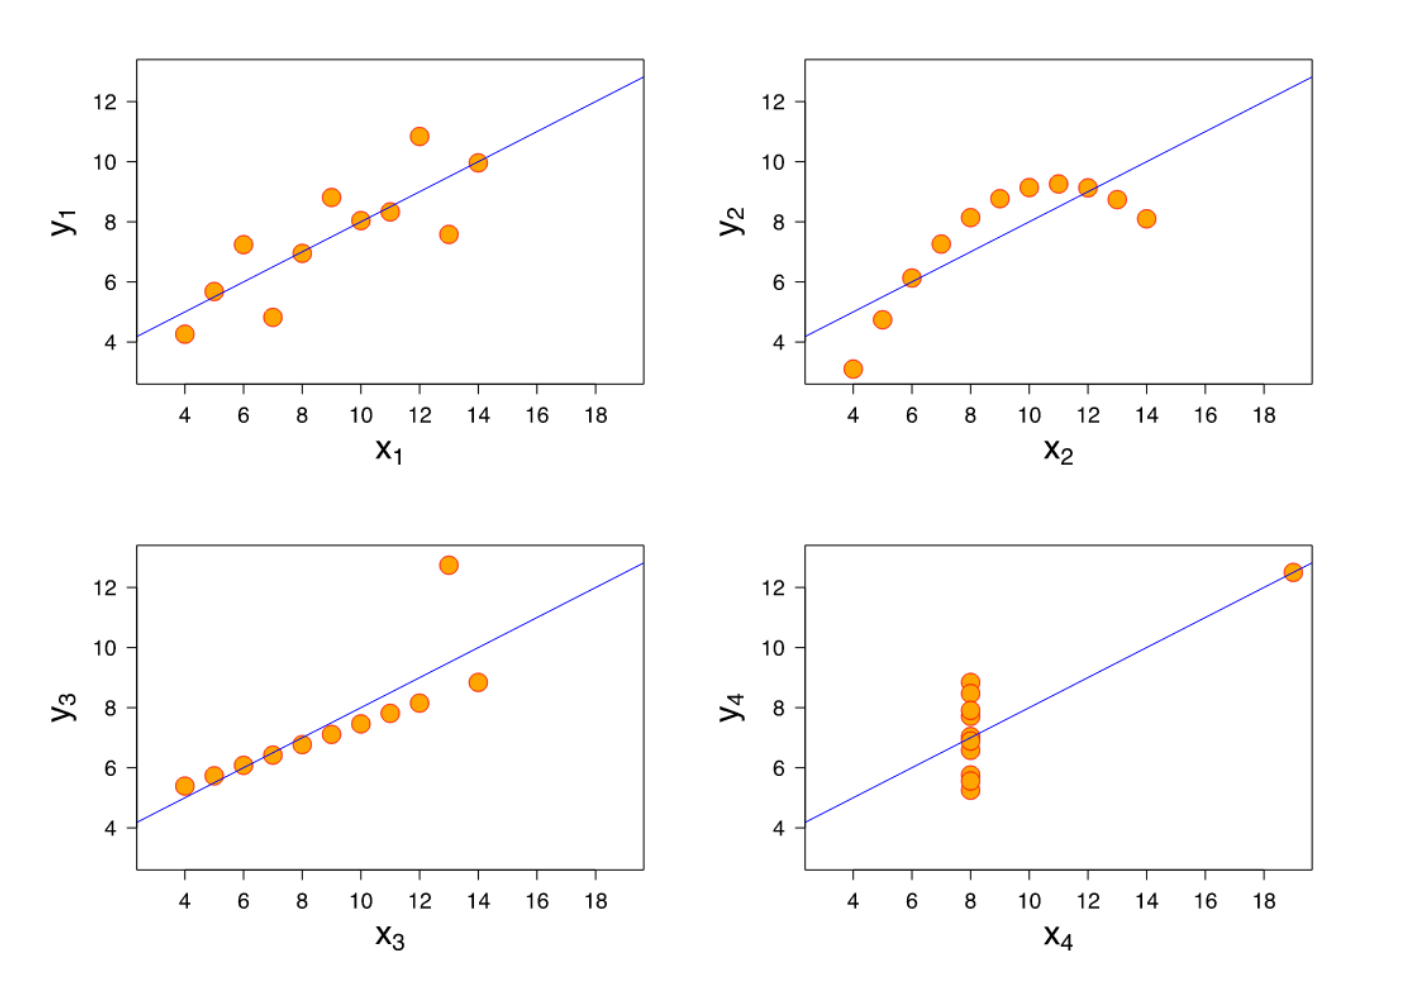
\includegraphics[scale=0.3]{quartet}
	 \end{center}
	\end{frame}

			\begin{frame} 
	\frametitle{\insertsection} 
	\begin{center}
		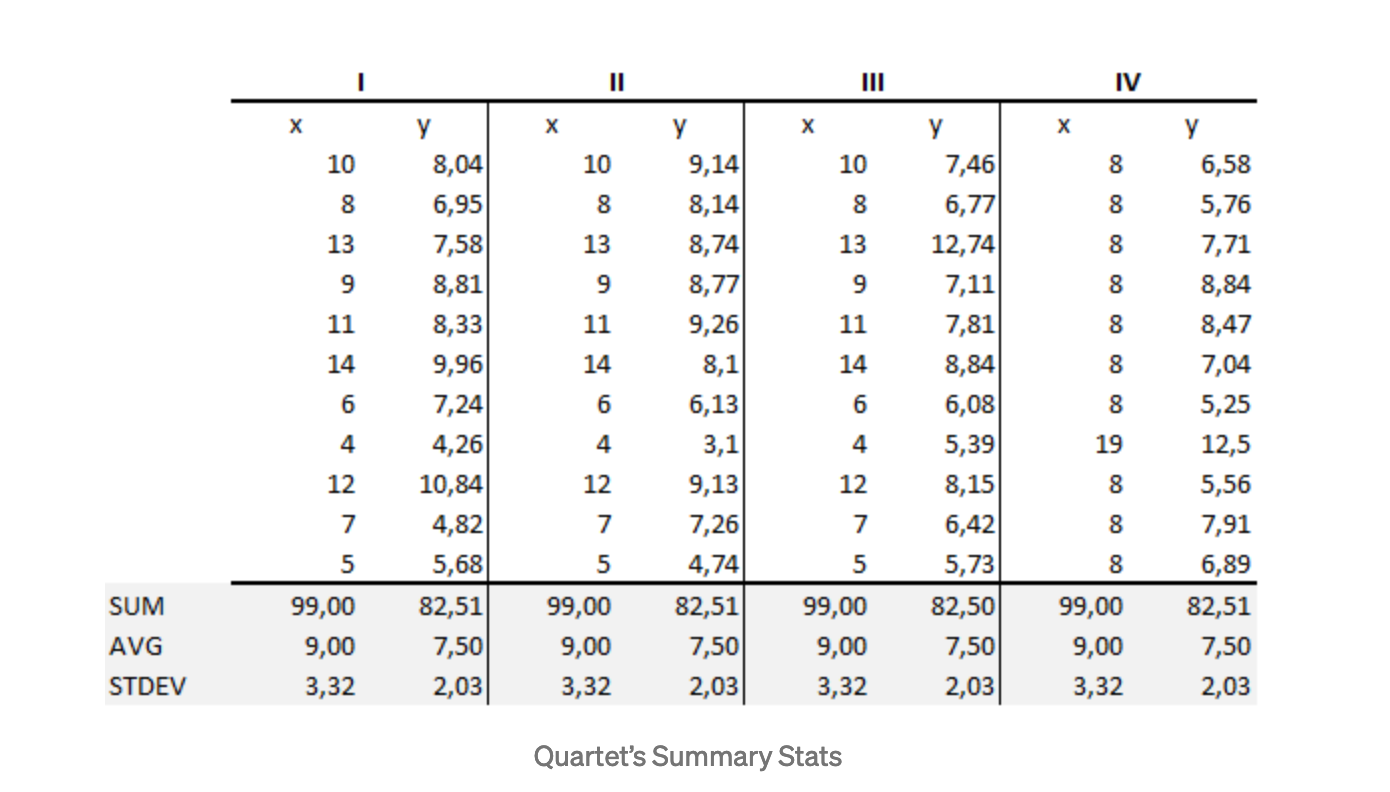
\includegraphics[scale=0.5]{stat_quart}
	\end{center}
\end{frame}

\section{Types}
		\begin{frame} 
		\frametitle{\insertsection} 
	Not sure that I  can do it better, let's just follow \href{https://towardsdatascience.com/top-16-types-of-chart-in-data-visualization-196a76b54b62}{this} link and discuss it. 
	\end{frame}

\section{Principles}
\begin{frame} 
	\frametitle{\insertsection} 
			\begin{itemize}
	\item Plot it's a story! 
	\item Choose type wisely! 
	\item Highlight important moments!
	\item Choose right colors!
	\item Pay attention to axes! 
	\item Pay attention to titles!
	\item Fancy does not mean cool
	\item Avoid redundancy, just important things on plot
	\item Add interactivity when appropriate
\end{itemize}
\end{frame}	

\section{Examples}
\begin{frame} 
	\frametitle{\insertsection} 
	\begin{center}
	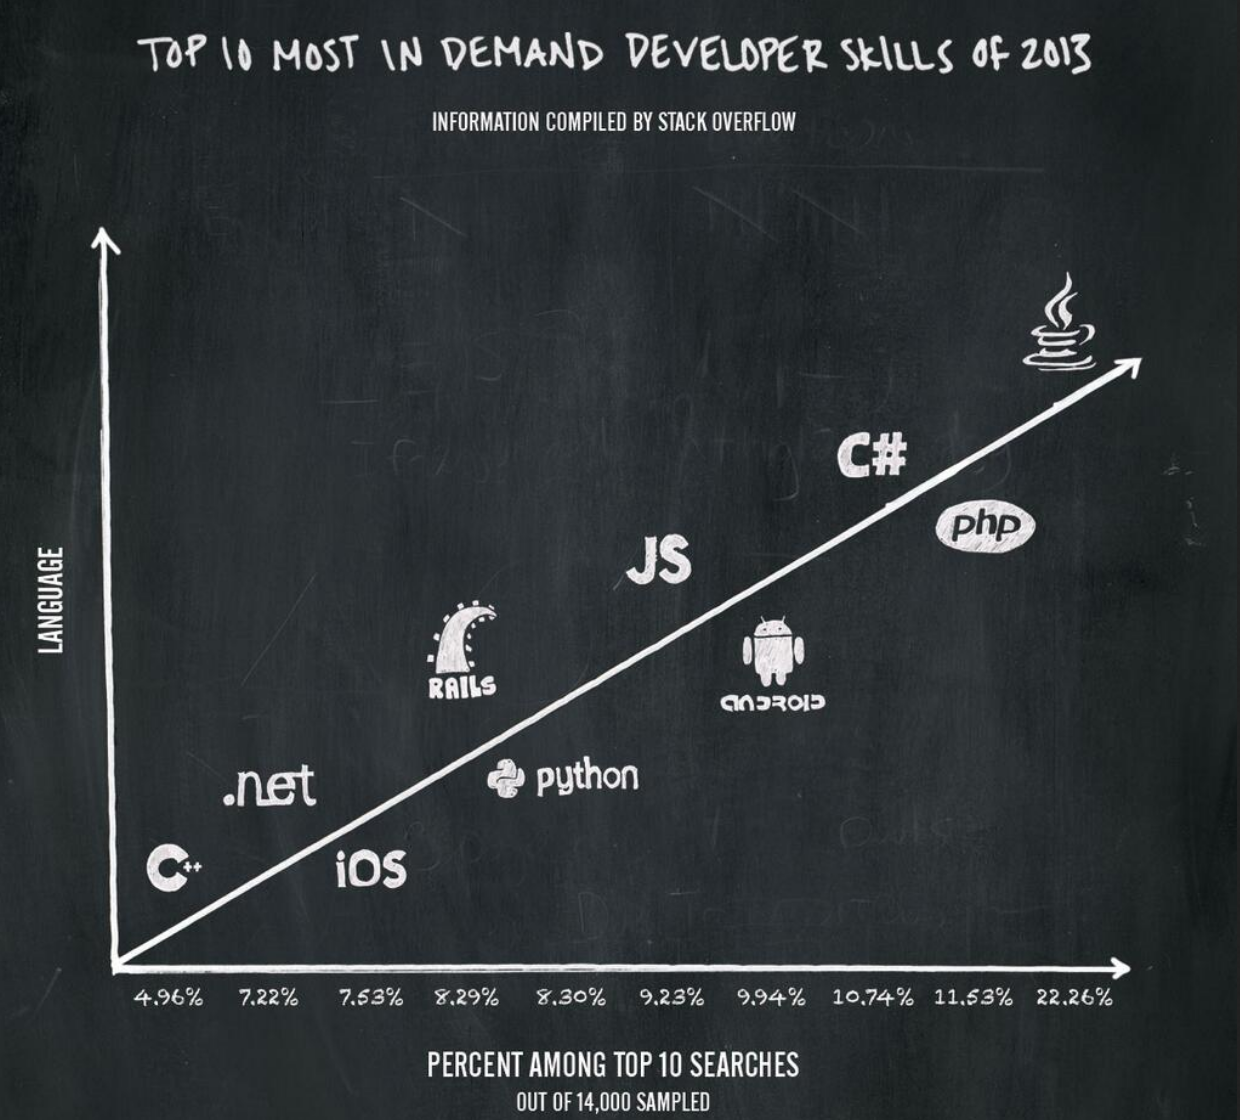
\includegraphics[scale=0.4]{bad_dev_plot}
\end{center}
\end{frame}

\begin{frame} 
	\frametitle{\insertsection} 
	\begin{center}
		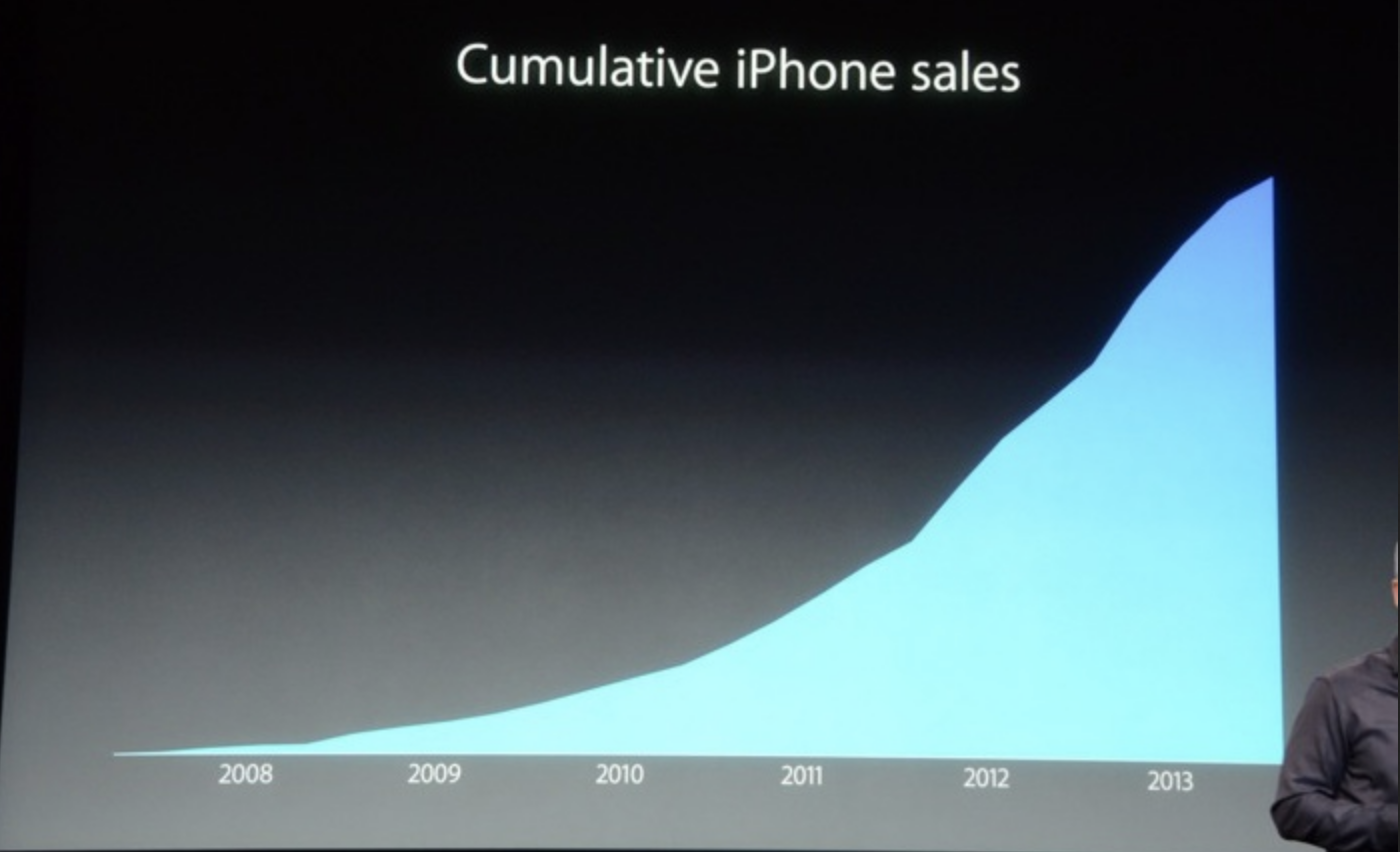
\includegraphics[scale=0.4]{iphone}
	\end{center}
\end{frame}

\begin{frame} 
	\frametitle{\insertsection} 
	\begin{center}
		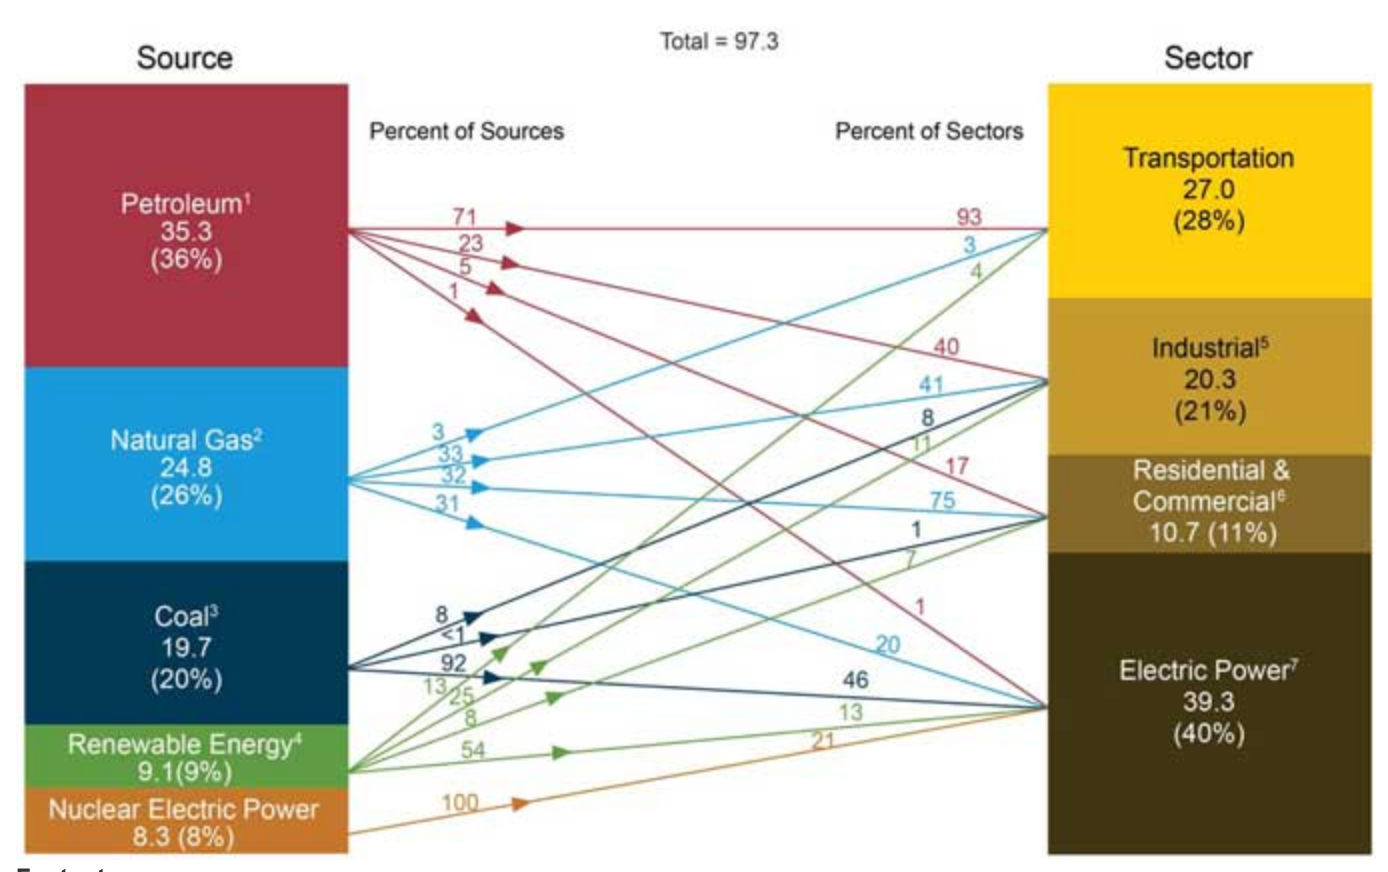
\includegraphics[scale=0.4]{bad_sankey}
	\end{center}
\end{frame}

\begin{frame} 
	\frametitle{\insertsection} 
	\begin{center}
		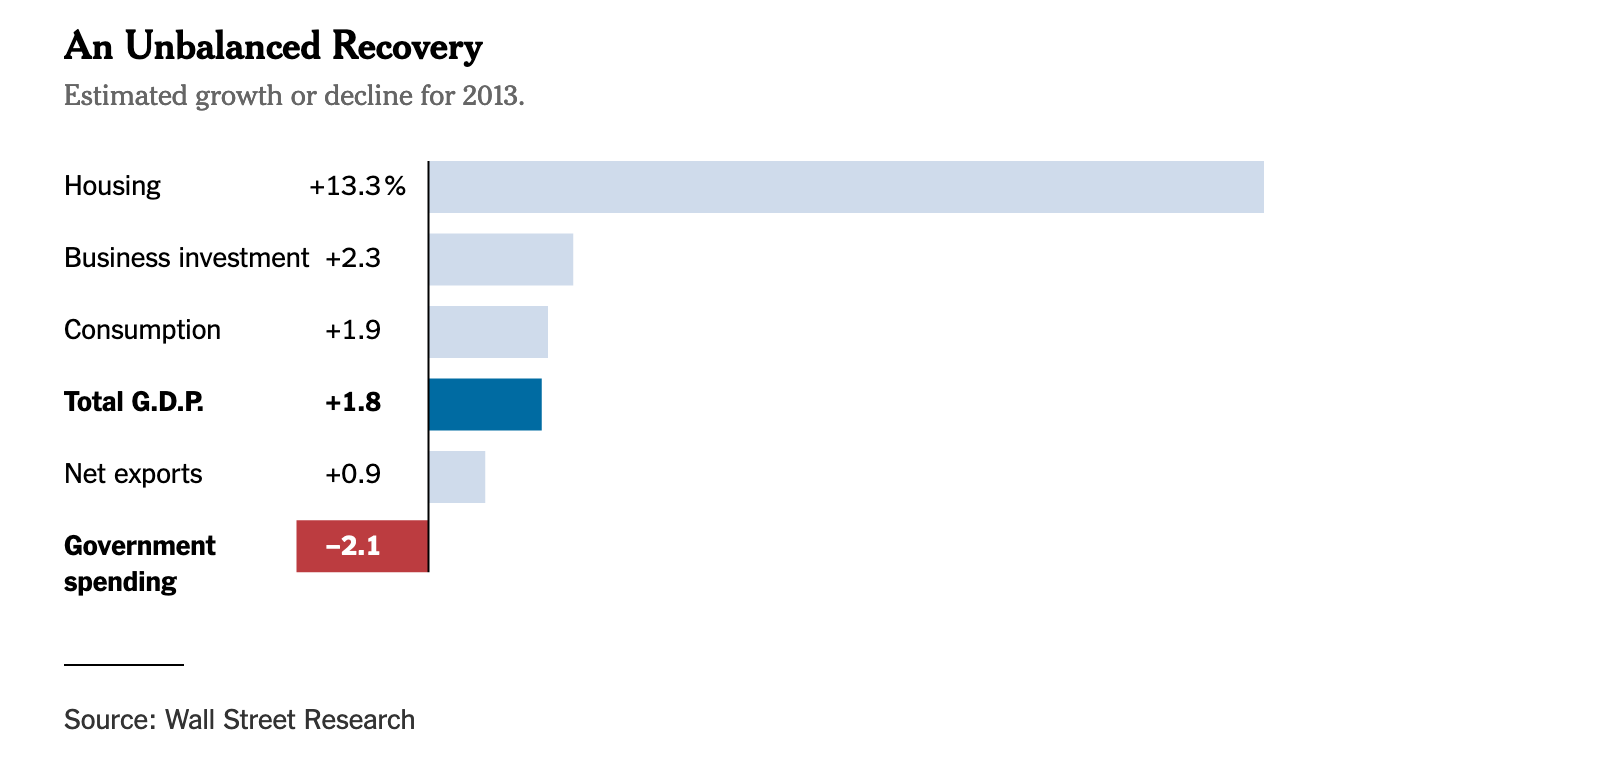
\includegraphics[scale=0.5]{good1}
	\end{center}
\end{frame}

\begin{frame} 
	\frametitle{\insertsection} 
	\begin{center}
		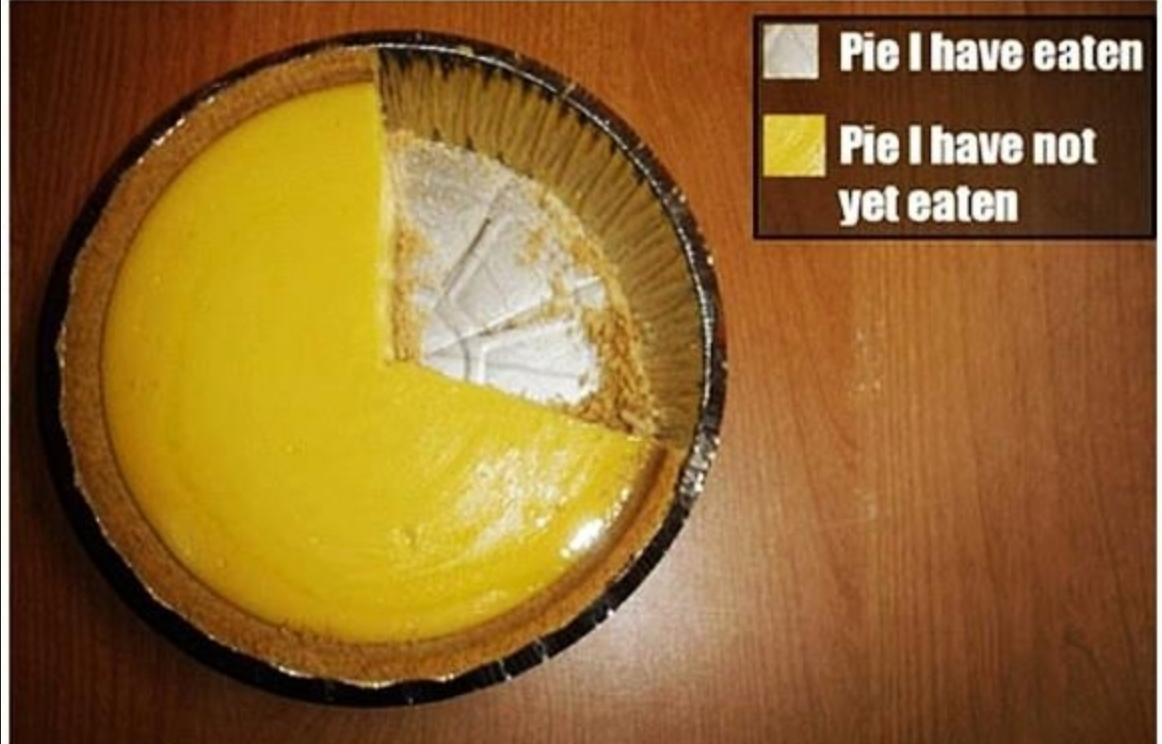
\includegraphics[scale=0.5]{goodpie}
	\end{center}
\end{frame}

\begin{frame} 
	\frametitle{\insertsection} 
	\begin{center}
		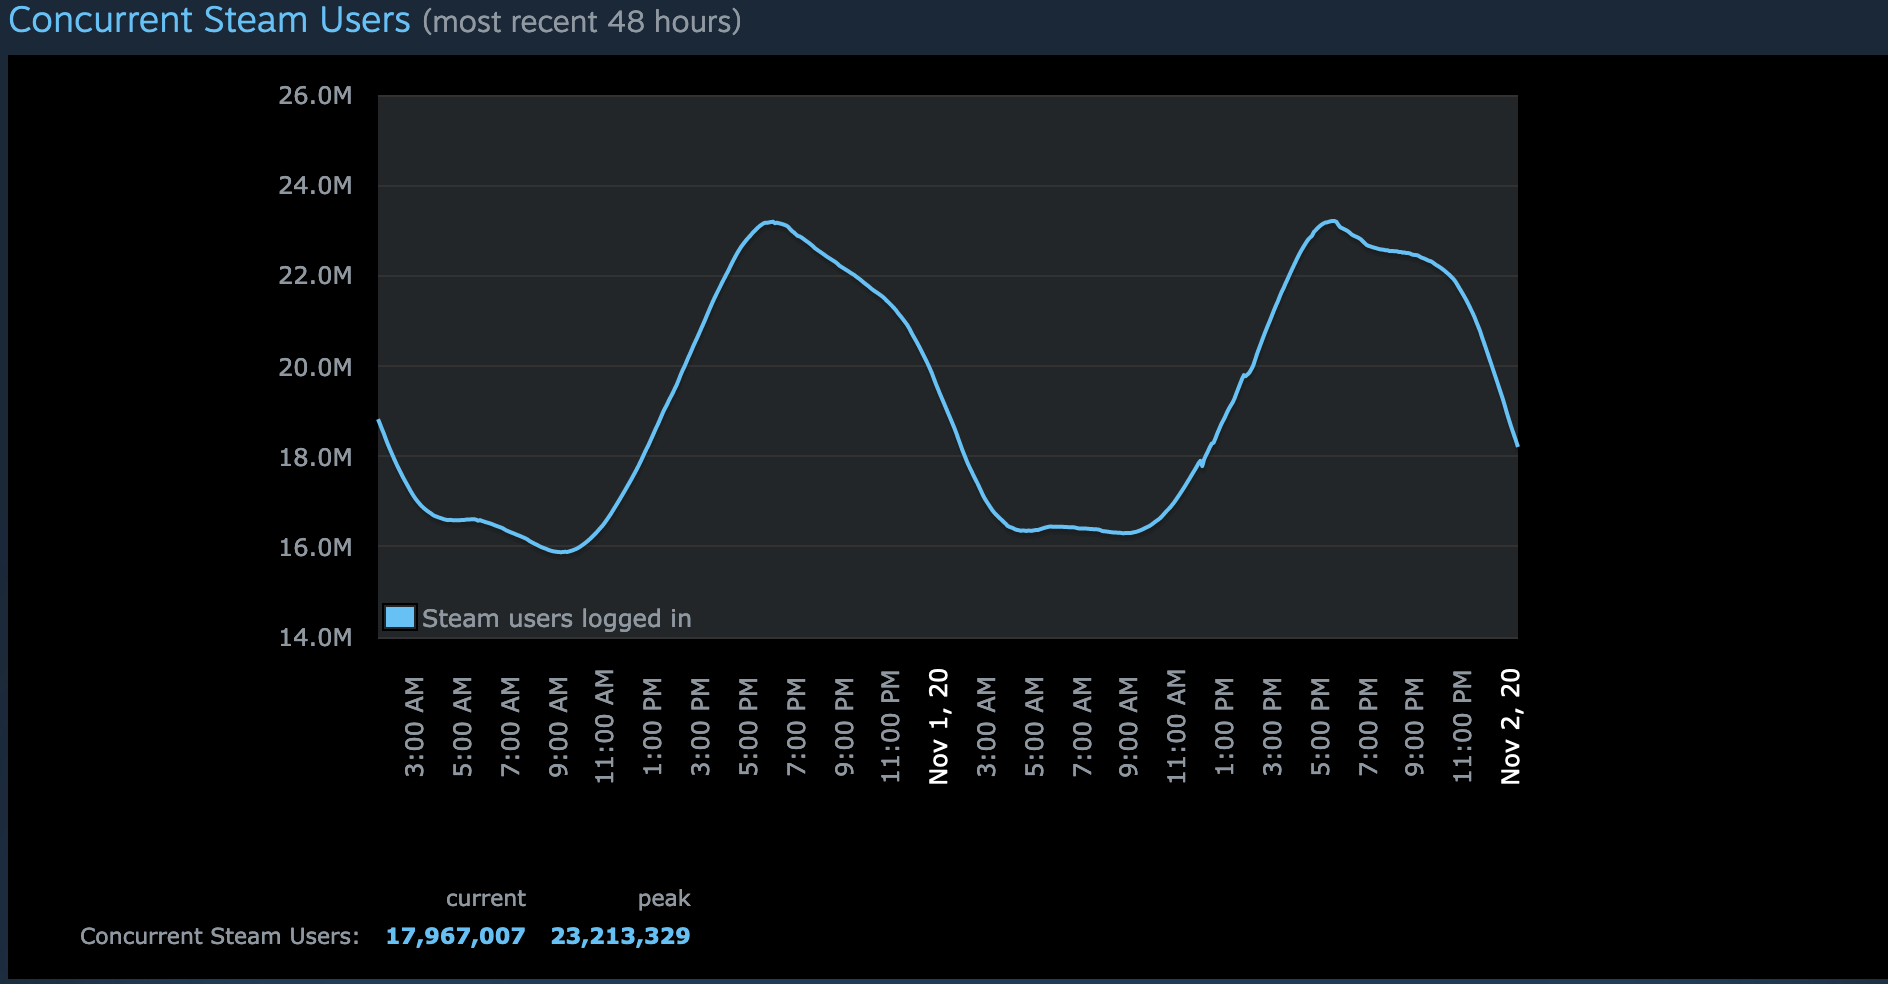
\includegraphics[scale=0.3]{goodsteam}
	\end{center}
\end{frame}

\begin{frame} 
	\frametitle{\insertsection} 
	\begin{center}
		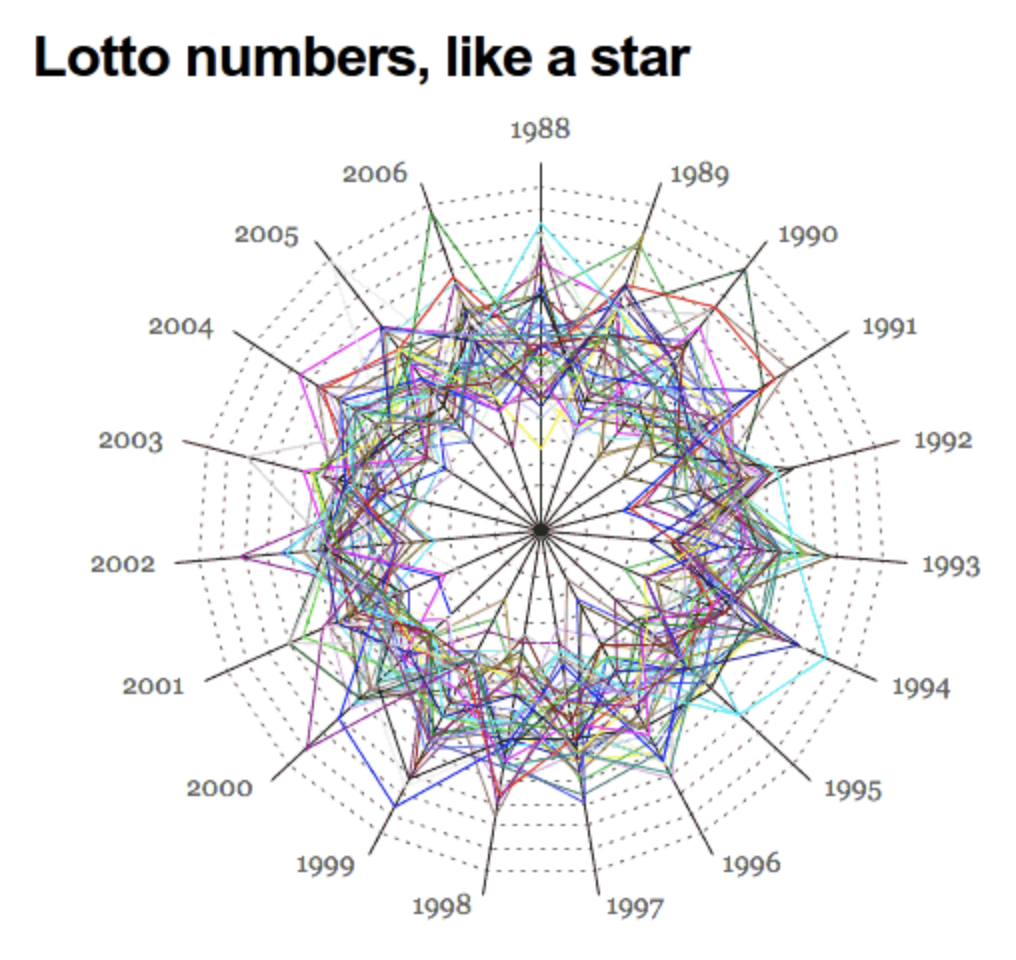
\includegraphics[scale=0.4]{messy_plot}
	\end{center}
\end{frame}

\end{document}